% !TEX TS-program = pdflatex
% !TEX encoding = UTF-8 Unicode

% This is a simple template for a LaTeX document using the "article" class.
% See "book", "report", "letter" for other types of document.

\documentclass[14pt]{article} % use larger type; default would be 10pt
\usepackage[14pt]{extsizes}
\usepackage[utf8]{inputenc} % set input encoding (not needed with XeLaTeX)
\usepackage[T2A]{fontenc}  %поддержка кириллицы в ЛаТеХ

\usepackage[titletoc]{appendix}
%%% Examples of Article customizations
% These packages are optional, depending whether you want the features they provide.
% See the LaTeX Companion or other references for full information.

%%% PAGE DIMENSIONS
\usepackage{geometry} % to change the page dimensions
\geometry{a4paper} % or letterpaper (US) or a5paper or....
\geometry{left=30mm, top=20mm, bottom=20mm, right=15mm} % for example, change the margins to 2 inches all round
% \geometry{landscape} % set up the page for landscape
%   read geometry.pdf for detailed page layout information

\usepackage[final]{graphicx} % support the \includegraphics command and options
\usepackage{epstopdf}
\let\bibsection\relax
\usepackage{amsmath}

%\usepackage[parfill]{parskip} % Activate to begin paragraphs with an empty line rather than an indent


%%% PACKAGES
\usepackage{amsfonts} %for \mathbb
\usepackage{amssymb}
\usepackage{dsfont}
\usepackage{booktabs} % for much better looking tables
\usepackage{array} % for better arrays (eg matrices) in maths
\usepackage{paralist} % very flexible & customisable lists (eg. enumerate/itemize, etc.)
\usepackage{verbatim} % adds environment for commenting out blocks of text & for better verbatim
\usepackage{subfig} % make it possible to include more than one captioned figure/table in a single float
\usepackage[english, russian]{babel}
\usepackage[hidelinks]{hyperref}
\usepackage{bookmark}
\usepackage{euscript}
\usepackage{caption}
\usepackage{pbox}
\usepackage[square,numbers]{natbib}
\setcitestyle{authoryear, open={[},close={]}}
% These packages are all incorporated in the memoir class to one degree or another...
%\usepackage{tempora}
\let\bibhang\relax
\let\citename\relax
\let\bibfont\relax
\let\Citeauthor\relax
\let\bibsection\relax
\expandafter\let\csname ver@natbib.sty\endcsname\relax
\usepackage[backend=bibtex,style=numeric]{biblatex}  %backend=biber is 'better'  

\addbibresource{kursach.bib}

\graphicspath{{img/}}

\usepackage{amsmath}
\usepackage{amstext}
%\usepackage{amssymb}
%\usepackage{bm}
%\usepackage{caption}
%\usepackage{color}
%\usepackage{epigraph}
%\usepackage{epsfig}
%\usepackage{float}
%\usepackage{gensymb}
%\usepackage{graphicx}
%\usepackage{hyperref}   
%\usepackage{mathtools}
%\usepackage{lipsum}
%\usepackage{indentfirst,latexsym}
%\usepackage{physics}
%\usepackage{setspace}
%\usepackage{subcaption}

%\onehalfspacing

\usepackage{xspace}

%%% HEADERS & FOOTERS
\usepackage{fancyhdr} % This should be set AFTER setting up the page geometry
\pagestyle{fancy} % options: empty , plain , fancy
\renewcommand{\headrulewidth}{0pt} % customise the layout...
\lhead{}\chead{}\rhead{}
\lfoot{}\cfoot{\thepage}\rfoot{}

%%% SECTION TITLE APPEARANCE
%\usepackage{sectsty}
%\allsectionsfont{\sffamily\mdseries\upshape} % (See the fntguide.pdf for font help)
% (This matches ConTeXt defaults)

%%% ToC (table of contents) APPEARANCE
\usepackage[nottoc,notlof,notlot]{tocbibind} % Put the bibliography in the ToC
\usepackage[titles,subfigure]{tocloft} % Alter the style of the Table of Contents
\renewcommand{\cftsecfont}{\rmfamily\mdseries\upshape}
\renewcommand{\cftsecpagefont}{\rmfamily\mdseries\upshape} % No bold!
\linespread{1.5}

\usepackage{indentfirst}

%%% END Article customizations



%\textheight 25.7cm % 29.7-2-2=25.7
%\textwidth 17cm % 21-2.5-1.5=17.0
%\hoffset -0.04cm %2.5-2.54=-0.04 слева 3см
%\voffset -1.04cm %2-2.54=0.54 сверху 2см
%\oddsidemargin 0cm
%\headheight 0cm
%\headsep 0cm
%\topmargin 0cm
%\setcounter{page}{1}
\def\sigspace{\\[1em]
\underline{\hspace{5cm}}\\[-0.2em]}

\begin{document}

\begin{titlepage}
	\begin{center}
		{
		{\bf Санкт-Петербургский Государственный Университет\\
		\vskip 1em
		Математико-механический факультет\\
		Кафедра Астрономии} }

	\vspace{3cm}
    	
	{\large А.С.\,Патшин}
    
    \vskip 2em
    

	\Large{\bf{Сравнение тригонометрических параллаксов звезд TGAS и Hipparcos}}
    \vskip 1em
    {\normalsize {Дипломная работа}\\}
	\end{center}
	
	\vskip 5em
    
	{
		 \begin{flushright}
			Научный руководитель:\\
		    доцент А.С.\,Цветков \sigspace
		    Рецензент:\\
		    PhD. З.М.\,Малкин \sigspace
		\end {flushright}
	}

	\vfill
	\begin{center}
	\small {Санкт-Петербург

	2018}
	\end{center}
\end{titlepage}

\newpage
\begin{titlepage}
	\begin{center}
		{
		{\bf Saint-Petersburg State University\\
		\vskip 1em
		Mathematics and Mechanics Department\\
		Chair of Astronomy} }

	\vspace{3cm}
    	
	{\large Anton Patshin}
    
    \vskip 2em
    

	\Large{\bf{Comparison of trigonometric parallaxes of TGAS and Hipparcos stars}}
    \vskip 1em

    {\normalsize {Graduation Thesis}\\}
	\end{center}
	
	\vskip 5em
    
	{
		 \begin{flushright}
			Scientific supervisor:\\
		    associate professor Alexander Tsvetkov \sigspace
		    Reviewer:\\
		    PhD. Zinovy Malkin \sigspace
		    
		\end {flushright}
	}

	\vfill
	\begin{center}
	\small {Saint-Petersburg

	2018}	
\end{center}
\end{titlepage}
\newpage
\tableofcontents
\newpage



 
\section{Введение}\label{introduction}

(Переписать этот пример под мою работу)


Сравнение каталогов является класической задачей фундаментальной\\ астрометрии, производщей переход от отдной системы координат к другой, оценить уровень систематических ошибок. До недавненго времени могло проводиться сравнение лишь положений и собственных движений.Появление первых результатов миссии GAIA, в частности, каталога TGAS, позволило впервые проихвести сравение тригонометрических параллаксов общих звезд каталогов TGAS и  Hipparcos, а именно его второй версии XHIP (XHIP: An extended hipparcos compilation, Anderson, 2012). Каталог TGAS содержит 2057050 звезд с данными о тригонометрических параллаксах, включает в себя только звезды Hipparcos и Tycho-2  и не является в полном смысле независимым продуктом, т.к. использует в качестве первой эпохи данные этих двух каталогов. Для сравнения мы используем общие звезды XHIP  и TGAS, которых оказалось 93635,из 117954 ожидаемых. из которыз пригодно для анализа 90283.

\subsection{Общие сведенья о GAIA и TGAS}\label{sub:smthgaia}
Каталог GAIA
		
\subsection{Общие сведенья о Hipparcos}\label{sub:smthhip}
Тут мой супер классный диплом
$https://www.cosmos.esa.int/web/hipparcos/catalogue-summary$
$http://www.astronet.ru/db/msg/1210304/node2.html$

\subsection{Постановка задачи}\label{sub:smthzd}
	Сравнение параллаксов.\\
Возможно два варианта, что подобные результаты могут быть случайными выбросами или систематическими разностями.

\subsection{Выборка}\label{sub:smthzd}
Благодаря тому, что у каждой звезд в каталоге TGAS есть идентификатор из каталога Hipparcos (в противном случае из каталога Tyho-2), мы можем объединить данные по этим звездам с данными из каталога Hipparcos. Таким образом в объединённом каталоге будут данные из каталога XHIP и TGAS. В каталоге XHIP 117955 объектов. В TGAS 2057050. их объединении по звездам-- 93635, из котрых пригодны для анализа тригонометрических параллаксов  90283.


Перечислим интересующие нас поля из каждого каталога XHIP:

\begin{itemize}

\item $id$ - идентификатор звезды в каьалогк Hipparcos

\item $\pi_{xhip}$ - абсолютный барцентрический параллакс звезды на момент эпохи каталога, указано в mas

\item $\delta_{\pi_{xhip}}$ - стандартное отклонение параллаксов звезды на момент эпохи каталога, указано в mas

\end{itemize}

Из каталога TGAS нас интересуют следующие поля

\begin{itemize}

\item $hip$ - идентификатор звезды в каталоге Hipparcos

\item $\pi_{tgas}$ - абсолютный барцентрический параллакс звезды на момент эпохи каталога, указано в mas

\item $\delta_{\pi_{tgas}}$ - стандартное отклонение параллаксов звезды на момент эпохи каталога, указано в mas

\item $ra$ - экваториальна долгота на момент эпохи каталога, указано в градусах

\item $dec$ - экваториальна широты на момент эпохи каталога, указано в градусах

\item $l$ - галактическая долгота на момент эпохи каталога, указано в градусах

\item $b$ - галактическая широты на момент эпохи каталога, указано в градусах

\item $lon$ - эклиптическая долгота на момент эпохи каталога, указано в градусах

\item $lat$ - эклипическая широты на момент эпохи каталога, указано в градусах

\end{itemize}

\section{Построение и анализ разностей паралаксов}\label{errvid}
<Переписать>
Астрометрические каталоги за долгую историю сравнивали  всегда между собой с целью выявления случайных и особенно систематических ошибок на координаты и собственные движения. Впервые в истории появляется возможность сравнить параллаксы, полученные тригонометрическим способом для стоолько большого колличества звезд. К сожалению, параллаксы XHIP и TGAS  не являются независимыми величинами. Корректную процедуру сравнения удается сделать лишь после вызода покрайней мере GAIA DR2 (ссылка?), где параллаксы будут получены независимо от данных Hipparcos.

РАссмотрим для каждой звезды общего каталога величину разности параллаксов в XHIP и в TGAS, т.е. $\pi_{xhip} - \pi_{tgas}$. Ошибкой разности, соответственно, будем считать $\sqrt{\delta^2_{\pi_{xhip}} + \delta^2_{\pi_{tgas}}}$. Для начала выпишем различные статистические характеристики данной величины. СРеднее значение - 0.35 mas, Медиана 0.29, Стандартное отклонение -- 1.5 mas, Среднее значение подуля -- 1.04 mas, Медиана модуля - 0.76 mas, 99 персентиль модуля - 4.78 mas. 

Обычно систематические разности положений и собственных движений изучают в эквивалентной, в силу зонного построения каталогов, или гfлактической системе для массивных звездных каталогов, в котрых распределение звезд в этой системе симметрично (ссылка на работы витязева и цветкова?). Первое знакомство с систематическими разностями параллаксов (пир 4), показывает.что присутствует имметрия разностей относительно эклиптики.

Боллее того, мы видим зависимость между модулем разности параллаксов на рис.4 и ошибкой параллаксов в XHIP на рис.6  в эклиптической системе координат. Действительно, коэффицент корреляции между этими величинами на звездах объего каталога равен 0.55. Это говорит о том, что чем выше ошибка параллаксоа XHIP, тем ссильнее он отличается от параллакса TGAS.

\section{Анализ больших выборосов}\label{errvid}
Рассмотрим звезды у которых параллаксы в XHIP и TGAS  значимо различаются, а именно, у которых модуль разности параллаксов больше, чем 3 ошибки этой разности. Таких звезд 2148. Выясним, с чем связаны такие отличия в параллаксах. У таких звезд поэффициент корреляции моуля разности параллаксов с ошибкой параллакса в XHIP равен 0.87, а с ошибкой в TGAS -- 0.1. Т.е. можно утверждать. что большая разница медлу параллаксами обусловленна большими ошибками параллаксов именно в XHIP/ Явно ошибочными являются параллаксы меньше 0, т.е. этотакие паралаксы $\pi$ , что $\pi < -3\delta_{\pi}$. В TGAS таких звезд всего 6, а в XHIP - 17. Т.е. подобного рода выбросы не должны сильно влиять на усредненные характеристики разности параллаксов XHIP и TGAS.



\section{Случайные выбросы}\label{errvid}

\subsection{Проекция Хаммера}\label{sub:smthrs}

Hammer projection

Переход из сферических координат в координаты на проекции Хаммера

$$ x = \frac{2 \sqrt 2 \cos \varphi \sin \frac{\lambda}{2}}{\sqrt{1 + \cos \varphi \cos \frac{\lambda}{2}}} $$
$$y = \frac{\sqrt 2\sin \varphi}{\sqrt{1 + \cos \varphi \cos \frac{\lambda}{2}}}$$

Переход из координат проекции хамера в сферические координаты

$$z \equiv \sqrt{1 - \left(\tfrac14 x\right)^2 - \left(\tfrac12 y\right)^2}$$
$$ \lambda = 2 \arctan \frac{zx}{2\left(2z^2 - 1\right)} $$
$$ \varphi = \arcsin zy $$


\subsection{Распределение}\label{sub:smthrs}
Тут мой супер классный диплом

и супер классные картиновчки и гистограмки


\section{Анализ разностей с помощью сферических функций}\label{sistem}
 На рис.4 мы видим явную зависимость в распределении модуля отличия параллаксов по небесной сфере от модуля эклиптической широты (коэффецент корреляции равен -0.7).  Подтвердить статистическую значимость данной зависимости и незначимость прочих менее оччевидных зависимостей мы можем с помощью представления пмодуля разностей параллаксов через сферические функции. Сферические функции широко используются в различных областях математики и физики, их определение можно найти во многих источниках (см., например, Арфкен, 1970). Впервые  были использованы для анализа систематических разностей положений и собственных движений (броше 1977). Мы впервые используем этот инструмент для анализа систематических разностей параллаксов.
 
Представление модуля разницы параллаксов с помощью линейной комбинации сферических функций можно записать следующим образом.

$$ \Delta_{plx} (l,b) = \sum_{nkp}\delta_{nkp}K_{nkp}(l,b) $$,
где сферические функции имеют вид (Арфкен, 1970):

$$ K_{nkp}(l,b) = R_{nk} $$


\section{Систематические различия}\label{sistem}
		

\subsection{Healpix}\label{sub:smthhealpix}
HEALPix -- это абревиатура \textbf{H}ierarchical \textbf{E}qual \textbf{A}rea iso\textbf{L}atitude \textbf{Pix}elation of a sphere (Иерархическая равная изоляционная площадь пикселей). 

Первоначальным мотивом для разработки HEALPix была мпутниковая миссия NASA (http://map.gsfc.nasa.gov/) сана по измерению <>, и в настоящее время действует миссия ESA Planck -- созданию полномасштабной карты реликтового излучения (микроволного анизотропного поля) с угловым разрешением несколько угловых секунд. Основными требования при разработке HEALPix, было создание математической структуры, которая поддерживает подходящую дискретизацию функций на сфере при достаточно высоком разрешении и облегчает быстрый и точный статистический и астрофизический анализ массивных наборов данных полного неба.

HEALPix удовлетворяет этим требованиям, поскольку обладает следующими тремя существенными свойствами:

\begin{itemize}
\item Сфера иерархически тесселирована в криволинейный четырёхугольник. Проекция с самым низким разрешением состоит из 12 базовых пикселей. Разрешение тесселяции увеличивается за счёт деления каждого пикселя на четыре новых. На следуюзщем рисунке показано (по часовой стрелке от верхнего левого до нижнего левого)разрешение увеличивается на 3 шага от базового уровня (т.е. сфера разделена соответственнно на 12, 48, 19 и 768 пикселей).
\item Области/Площади всех пикселей при заданном разрешении идентичны.
\item Пиксели распределены по линиям постоянной широты. Это свойство необходимо для всех приложений гармонческого анализа с участием сферических гармоник. Из-за изо-широтного распределения точек выборки скорость вычисления интегралов по отдельным сферическким гармоникам масштабируется как $~N^{1/2}$ с общим колличеством пикселей, в отличае от пасштабирования $~N$ для распределений выборки неизото-широты(?) (примерами которой является четырёхгранный сферический куб ($http://lambda.gsfc.nasa.gov/product/cobe/skymap_info_new.cfm$), используемый для COBE ($http://lambda.gsfc.nasa.gov/product/cobe$) NASA данные и любое распределение, основанное на симметрии икосаэдра).
\end{itemize}

\begin{figure}[h!]
\center{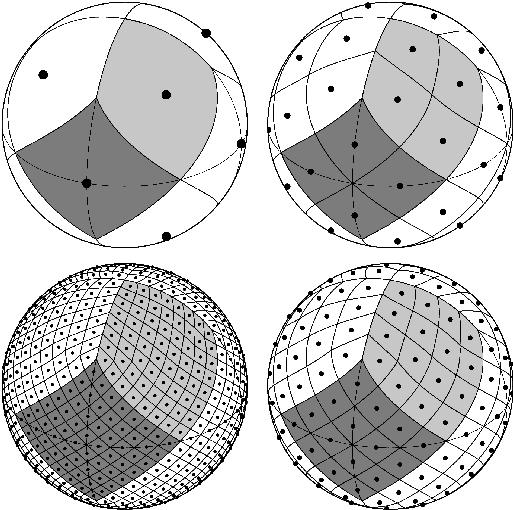
\includegraphics[width=0.5\linewidth]{healpix}}
\caption{Деление сферы на равные по пложади сигменты.}
\label{img:healpix}
\end{figure}

Как было предложено в названии, эта пикселизация создаёт сигменты сферической поверхности, в которой каждый пиксель покрывает ту же площадь поверхности, что и любой другой пиксель. На рисунке ниже представлено разбиение сферы пропрорционально более высокие разрешения слева на право. Зеленая сфера представлет собой самое минимальное разрешение, возможное при базаовом разбиении поверхности шара HEALPix на 12 пикселей равного размера. Желтая сфера имеет сетку HEALPix 48 пикселей, красная сфера -- 192 пикселя, а синяя сфера имеет сетку 768 пикселей (разрешение 7.3 градуса). Как не сложно догадаться, колличество пикселей можно посчитать по формуле $$NSIDE = 12*n^2, n \in \mathbb {N}$$.

\begin{figure}[h!]
\center{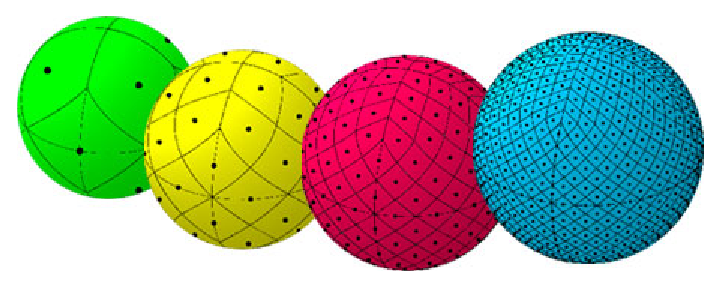
\includegraphics[width=1\linewidth]{healpixnasa}}
\caption{Разбиение HEALPix.}
\label{img:healpixnasa}
\end{figure}

Другим свойством сетки HEALPix является то, что пиксельные центы, представленные черными точками, встречаются на дискретном/конечном(?) числе колец постоянной широты, количество колец зависит от разрешения сетки HEALPix. Для примера, у зеленогой, желтой, красной и синей сферы их 3, 7, 15, 31 кольцо с постоянной широтой соответственно(?).

Ниже приведён пример применения HEALPix с высоким разрешением -- Модель реликтового излучения (CMB) (космическое сверхвысокочастотное фоновое излучение), состоящая из 12582912 пикселей (~ 3.4 минут дуги (arcmin)).


\begin{figure}[h]
\begin{minipage}[h]{0.3\linewidth}
\center{
\includegraphics[width=1\linewidth]{exampleCMB} \\На сфере}
\end{minipage}
\hfill
\begin{minipage}[h]{0.69\linewidth}
\center{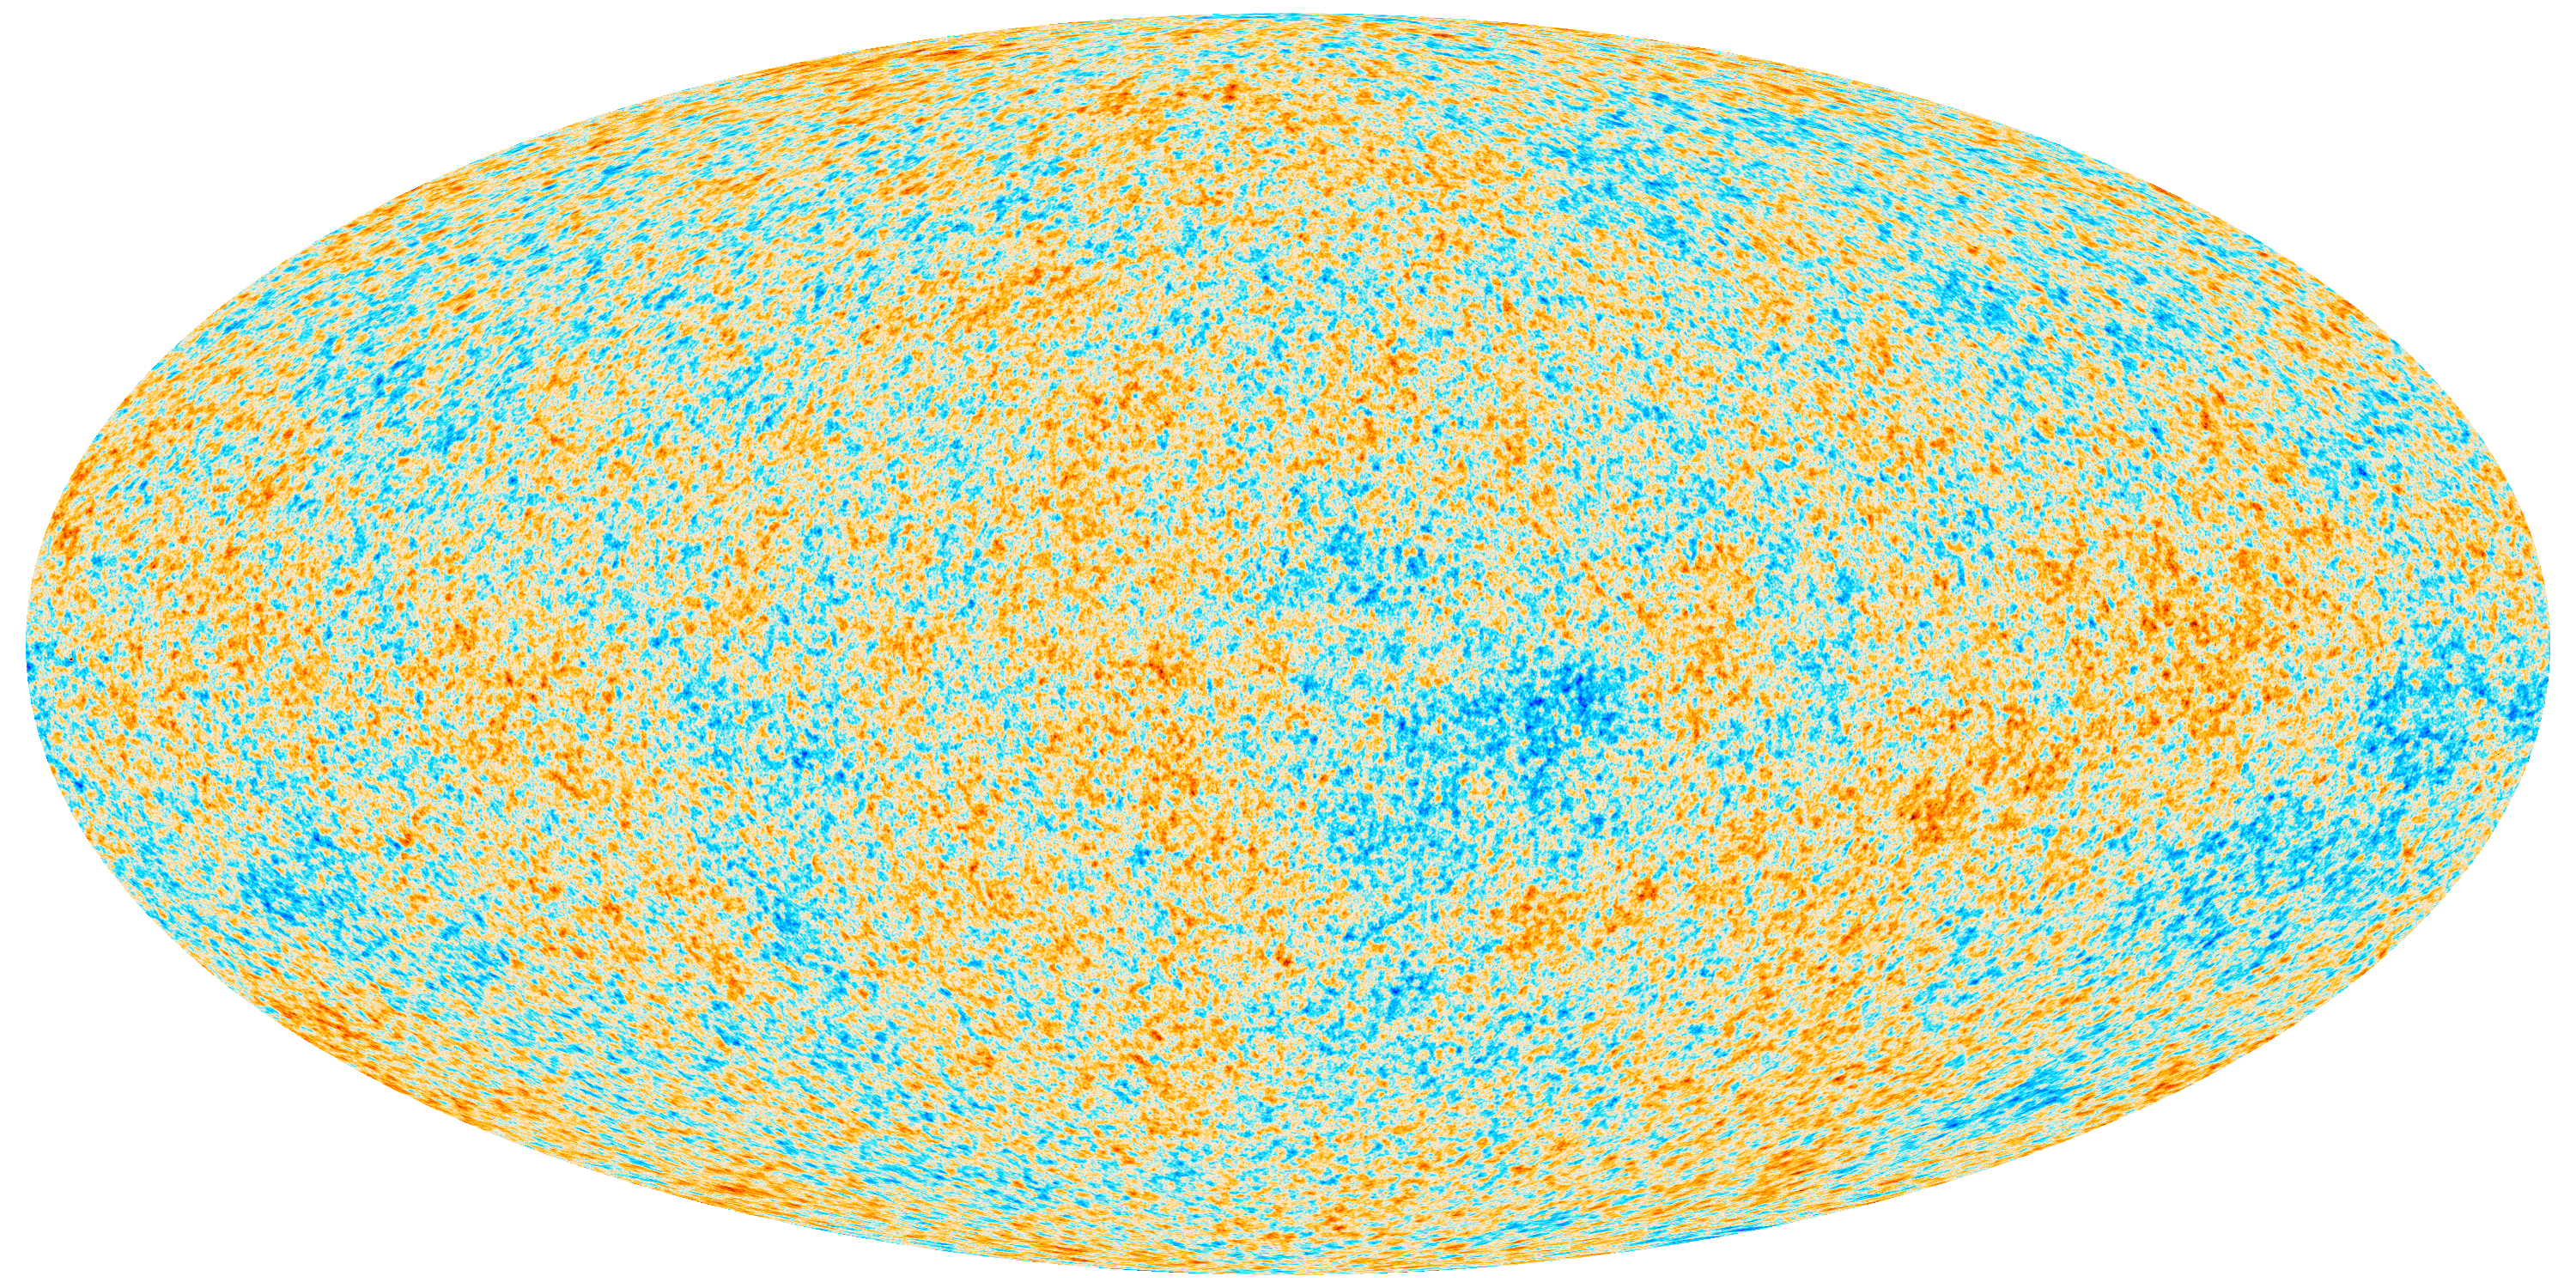
\includegraphics[width=0.85\linewidth]{planck2015_cmb_3000_cropped} \\Проекция Hammer}
\end{minipage}
\caption{Визуализация CMB на HEALPix}
\label{ris:image1}
\end{figure}


HealPix имеет два режима резбиения:
\begin{itemize}
\item NEST - позволяет работать со сферическими функциями и не только...

\item RING - позволяет определять минимальное расстояние до точек и не только...
\end{itemize}

\begin{figure}[h]
\begin{minipage}[h]{0.48\linewidth}
\center{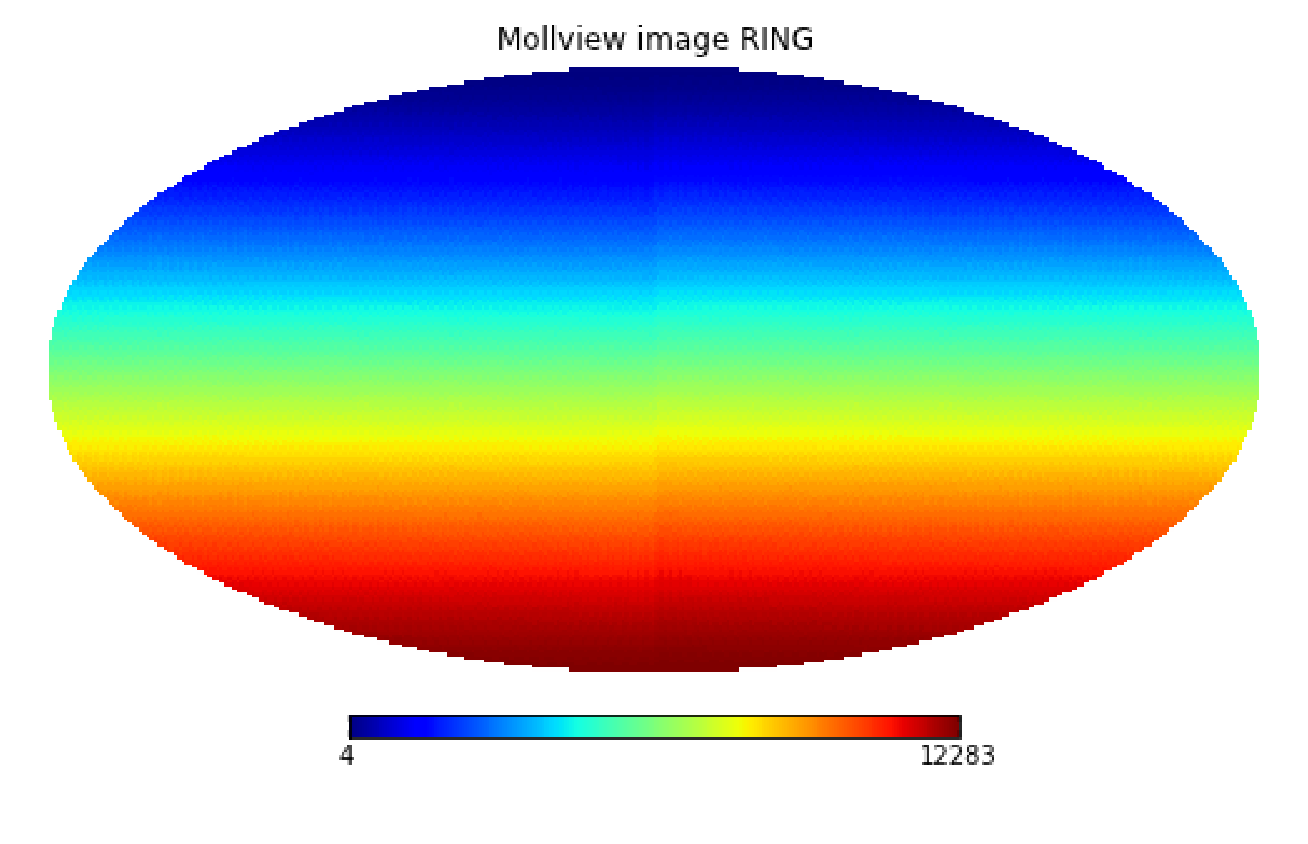
\includegraphics[width=1\linewidth]{moll_nside32_ring}}
\end{minipage}
\hfill
\begin{minipage}[h]{0.48\linewidth}
\center{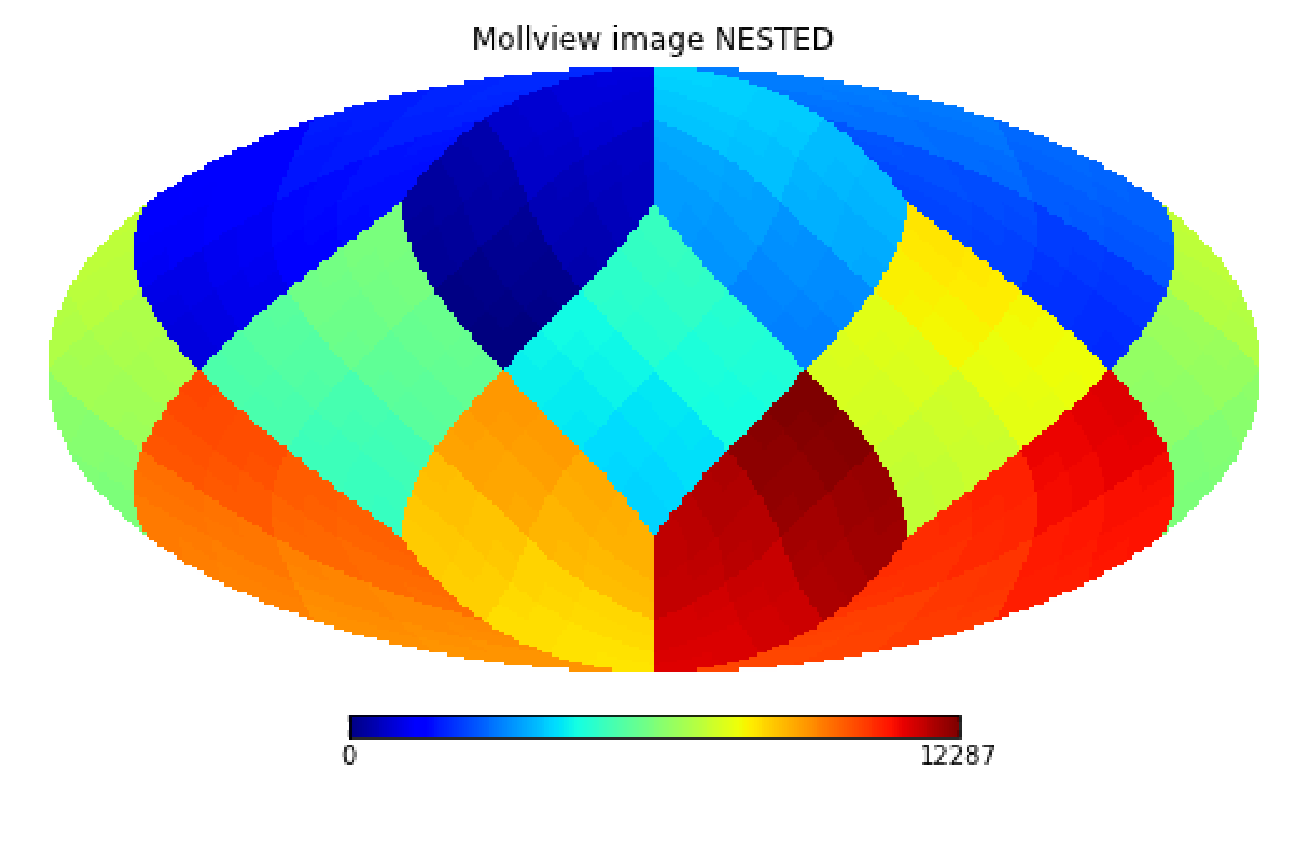
\includegraphics[width=1\linewidth]{moll_nside32_nest}}
\end{minipage}
\caption{Пример распределения  пикселей по ring and nest}
\label{ris:moll_nside32_healpix}
\end{figure}

Для нашей задачи отлично подходит NEST.

~\cite{wiki:healpix} 


Представление модуля разницы параллаксов с помощью линейной комбинации сферических функций.

$\delta_{plx}(l,b) = \sum_{nkp}\delta_{nkp}K_{nkp}(l,b)$

\subsection{Сферические функции}\label{sub:smthsf}
Сферичекие функции -- это очень полезный инстурумент при анализе небесной сферы ~\ref{img:sf} .
~\cite{book:sf}



$\sigma$



\begin{figure}[h!]
\center{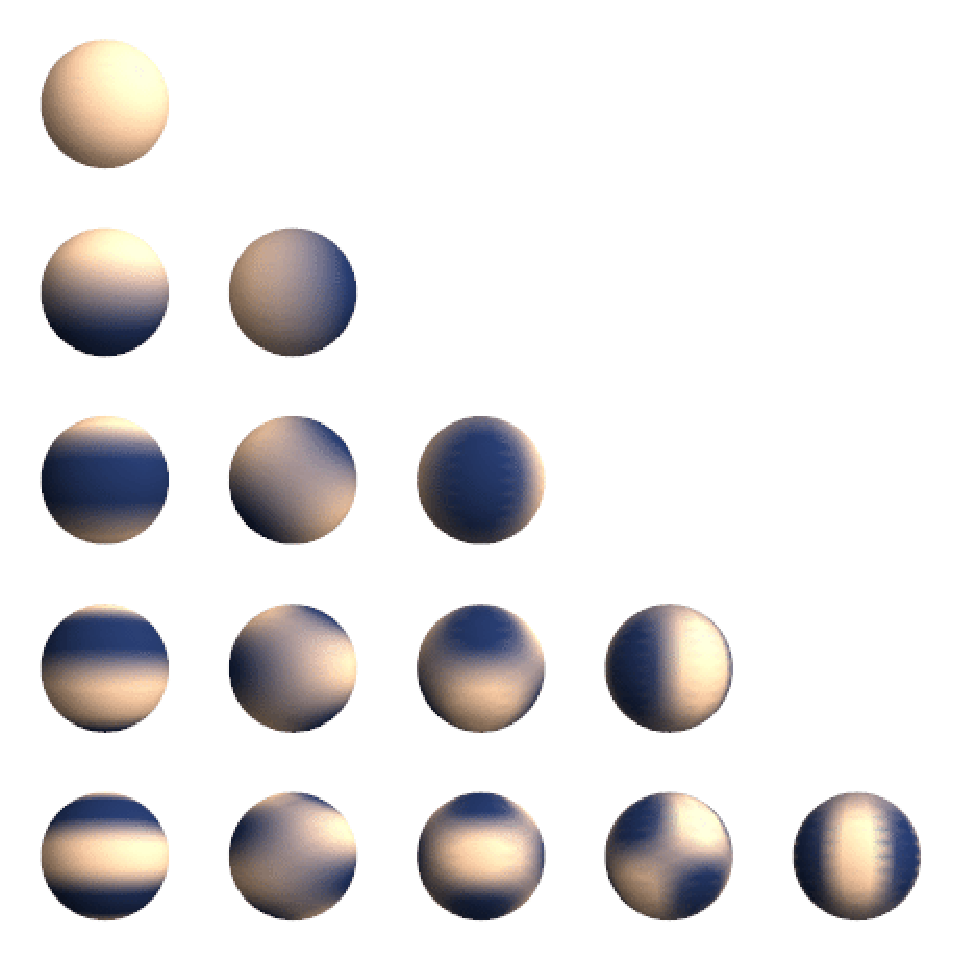
\includegraphics[width=0.5\linewidth]{Rotating_spherical_harmonics-0}}
\caption{Вещественные сферические функции $Y_{lm}$, $l=0…4$ (сверху вниз), $m=0…4$ (слева направо). Функции отрицательного порядка $Y_{l-m}$ повёрнуты вокруг оси Z на 90/m градусов относительно функций положительного порядка.}
\label{img:sf}
\end{figure}



\section{Заключение}\label{conclusion}
		ну вот и всё \cite{book:fourier} 

\newpage
\section{Список использованной литературы}\label{conclusionlit}
%\bibliographystyle{unsrt}
%\bibliography{kursach.bib}
\printbibliography[type=online,title={Online only}]
\printbibliography[type=book,title={Статьи:}]


\appendix

\section*{Приложение}
тут аппендикс или два 

\end{document}

